Muons are minimum-ionizing particle and are detected in the ATLAS detector through MS tracks or their characteristic energy deposits in the calorimeters. The primary reconstruction method for muons involve matching tracks in the MS to those in the ID\@. However, alternative reconstruction strategies exist for muons that only have tracks in a subset of the detectors subsystems.

Muon reconstruction begins by forming short straight-line track segments from hits in the MS stations. Segments are built by combining precision chamber hits with a Hough transform~\cite{ILLINGWORTH198887}. Track candidates are then created with segments from different stations in a loose fit based on the assumption that the muon originates near the IP and a first-order approximation on how much the muon bends in the magnetic field. A global $\chi^{2}$ fit is then applied on the muons trajectory through the magnetic field while accounting for material interactions and misalignments. Outlier hits are removed from the trajectory while additional hits along the trajectory are incorporated. Finally, another track fit is performed using the updated information.

Muon reconstruction consists of five main strategies leading to different muon types: combined (CB), inside-out combined (IO), muon-spectrometer extrapolated (ME), segment-tagged (ST), and calorimeter-tagged (CT). An illustration of these can be seen in Figure~\ref{fig:reco_muon_types}.
\begin{itemize}
  \item \textbf{Combined (CB):} These are identified using a fit combing hits in the ID and MS while taking into account energy loss in the calorimeters. Hits can be added or removed from the trajectory if it improves the fit quality. For $|\eta| > 2.5$, MS tracks can be combined with short track segments in the pixel and SCT detectors leading to a subset of these muons called silicon-associated forward (SiF) muons. CB muons account for 95\% of all reconstructed muons~\cite{ATLAS:2023iat}.
  \item \textbf{Inside-out combined (IO):} These are complementary to the CB muons and extrapolate ID tracks to the MS, searching for 3 MS hits that are loosely aligned. A fit is then performed using the ID, calorimeter energy loss, and MS tracks in a combined fit. These recover efficiencies in regions of limited MS coverage and low-$\pt$ muons.
  \item \textbf{Muon-spectrometer extrapolated (ME):} These are identified as hits in the MS without matching ID tracks. The MS hits are extrapolated to the beam-line to define a muon trajectory.\@. This method allows for the reconstruction of muons up to $|\eta| < 2.7$ which is beyond ID acceptance.
  \item \textbf{Segment-tagged (ST):} These are identified by extrapolating ID track to the MS and satisfy a tight angular matching to at least one MS segment. If matched, a fit is performed using the ID track fit parameters.
  \item \textbf{Calorimeter-tagged (CT):} These are identified by extrapolating ID tracks through the calorimeter searching for energy deposits consistent with a minimum-ionizing particle\@. If matched, a fit is performed using the ID track fit parameters.
\end{itemize}

\begin{figure}[hpt]
  \centering
  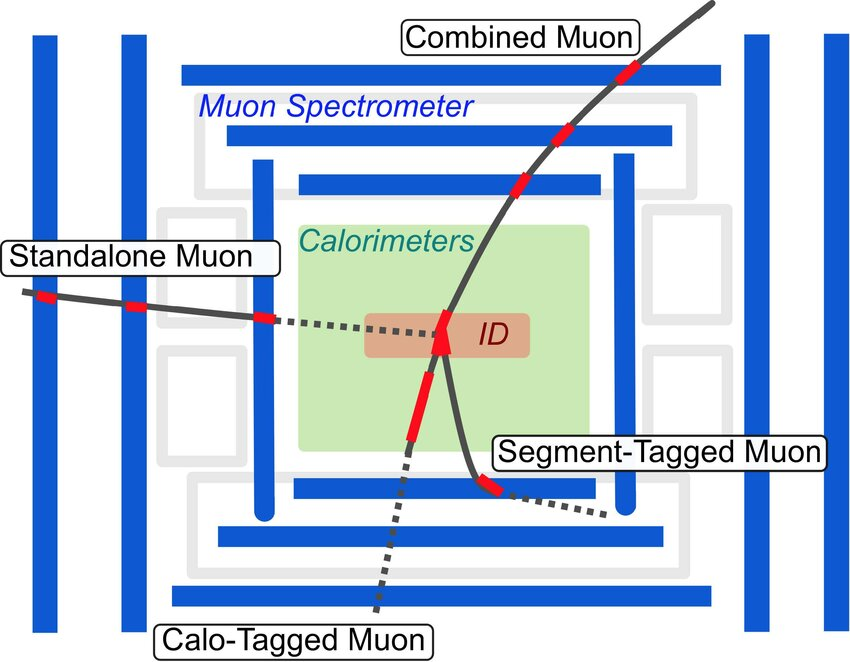
\includegraphics[width=0.65\textwidth]{figures/reco/reco_muon_reconstructions.jpg}
  \caption{Illustration of the different muon types reconstructed in the ATLAS detector. Taken from~\cite{Rettie:2018lly}.}\label{fig:reco_muon_types}. 
\end{figure}

More details about muon reconstruction can be found in Refs~\cite{ATLAS:2020auj, Rettie:2018lly, ATLAS:2023iat}.
